%!TEX program = xelatex
\documentclass[10pt]{beamer}
\usepackage{tikz}

\tikzset{global scale/.style={
    scale=#1,
    every node/.style={scale=#1}
  }
}
\setcounter{tocdepth}{1}
\usepackage{pgfplots}
\pgfmathdeclarefunction{gauss}{2}{%
  \pgfmathparse{1/(#2*sqrt(2*pi))*exp(-((x-#1)^2)/(2*#2^2))}%
}
\pgfplotsset{compat=1.10}

\def\x{-0.5}
\def\fx{1/(1.3*sqrt(2*pi))*exp(-((\x+0.5)^2)/(2*1.3^2))}
\def\y{1}
\def\fy{1/(0.9*sqrt(2*pi))*exp(-((\y-1)^2)/(2*0.9^2))}


\usetheme[menuwidth={0.7\paperwidth}]{erlangen}
\setbeamercovered{transparent=20}
\setbeamerfont{frametitle}{series=\bfseries}
\usepackage{hyperref}
\hypersetup{colorlinks=false,
            colorlinks=black,
            pdfborder=100,
            citecolor=black}


\setbeamerfont{block title}{series=\bfseries}
\usepackage{graphicx}


\usepackage[no-math,cm-default]{fontspec}
\setmainfont{Minion Pro}
\setsansfont[BoldFont={Myriad Pro Semibold}]{Myriad Pro}
\setmonofont{Courier New}
\usepackage{xeCJK}
\setCJKmainfont[BoldFont={方正黑体简体},ItalicFont={楷体}]{宋体}
\setCJKsansfont[BoldFont={方正黑体简体}]{方正中等线简体}
\setCJKmonofont{方正中等线简体}
\XeTeXlinebreaklocale "zh"
\XeTeXlinebreakskip = 0pt plus 1pt

\usefonttheme[onlymath]{serif}
\usepackage[noamssymbols]{mtpro2}

% \renewcommand\contentsname{目录}
\setbeamertemplate{itemize items}{\raisebox{0.15ex}{\small$\bullet$}}
\usetikzlibrary{matrix}
\begin{document}
\title{The International Diversification Puzzle Is Worse Than You Think}
\subtitle{Baxter and Jermann (AER, 1997)}
\author[Baxter and Jermann (AER, 1997)]{\today}
\date{\today}
% \institute{The School of Economics\\
  % \vspace{-0.2em}{\small Fudan University} }

\begin{frame}[plain]
  \titlepage
\end{frame}


\begin{frame}{Table of Contents}
  \tableofcontents
\end{frame}
\section{Introduction}
\section[Human Capital]{Human Capital and Portfolio Choice}
\section[Measuring]{Measuring Factor Returns}
\begin{frame}[c]\frametitle{Assumptions Relaxing}
\textbf{Privious Assumptions:}
\begin{itemize}
    \item factor shares constant;
    \item labor and capital returns are \alert{perfectly correlated};
\end{itemize}

\textbf{Assumptions Releasing:}
\begin{itemize}
    \item rich, short-term variation in factor shares;
    \item retaining the long-run restriction that factor shares are stationary;
    \item ratio of labor income to capital income is stationary;
    \item log of labor income and the log of capital income are cointegrated, and that the cointegrating vector is [1, -1].
\end{itemize}

\end{frame}

\begin{frame}[c]\frametitle{Econometric Model}
\begin{itemize}
    \item Based on these considerations, We estimate the following vector error correction model (VECM) for labor and capital income:
\end{itemize}
\begin{equation*}\small
    \begin{bmatrix}
    \Delta d_{L,t+1}\\
    \Delta d_{K,t+1}
    \end{bmatrix}
    =
    \begin{bmatrix}
    \delta_{L}\\
    \delta_{K}
    \end{bmatrix}
    +\begin{bmatrix}
    \psi_{LL}(L) & \psi_{LK}(L)\\
    \psi_{KL}(L) & \psi_{KK}(L)
    \end{bmatrix}\begin{bmatrix}
    \Delta d_{Lt}\\
    \Delta d_{Kt}
    \end{bmatrix}+\begin{bmatrix}
    \eta_{L}\\
    \eta_{K}
    \end{bmatrix}(d_{Lt}-d_{Kt}) + \begin{bmatrix}\varepsilon_{L,t+1}\\ \varepsilon_{K,t+1}\end{bmatrix}
\end{equation*}
where
\begin{itemize}
    \item $d_{Lt}$ denotes the log of labor income;
    \item $d_{Kt}$ denotes the log of capital income;
    \item $\Delta d_{L,t+1} \equiv d_{L,t+1}-d_{Lt}$;
    \item $\psi_{i,j}(L)$ are polynomials in the lag operator, $L$.
\end{itemize}

\end{frame}

\begin{frame}[c]\frametitle{Econometric Model II}
\textbf{Data:}
\begin{itemize}
    \item OECD National Accounts for Japan, Germany, the United Kingdom, and the United States: 1960--1993(anual);
    \item  measure of labor income: total employee compensation;
    \item measure of capital income: GDP at factor cost - employee compensation.
\end{itemize}
Assume that expected returns are constant over time (Campbell and Shiller 1988).
\begin{align}
    r_{t,t+1}^{L} - E(r_{t,t+1}^{L}) &= (E_{t+1}-E_{t})\big(\sum_{j=1}^{\infty} \rho^{j}\Delta d_{L,t+1+j}\big)\\
    r_{t,t+1}^{K} - E(r_{t,t+1}^{K}) &= (E_{t+1}-E_{t})\big(\sum_{j=1}^{\infty} \rho^{j}\Delta d_{K,t+1+j}\big)
\end{align}

\end{frame}

\begin{frame}[c]\frametitle{Results I:}

\begin{center}
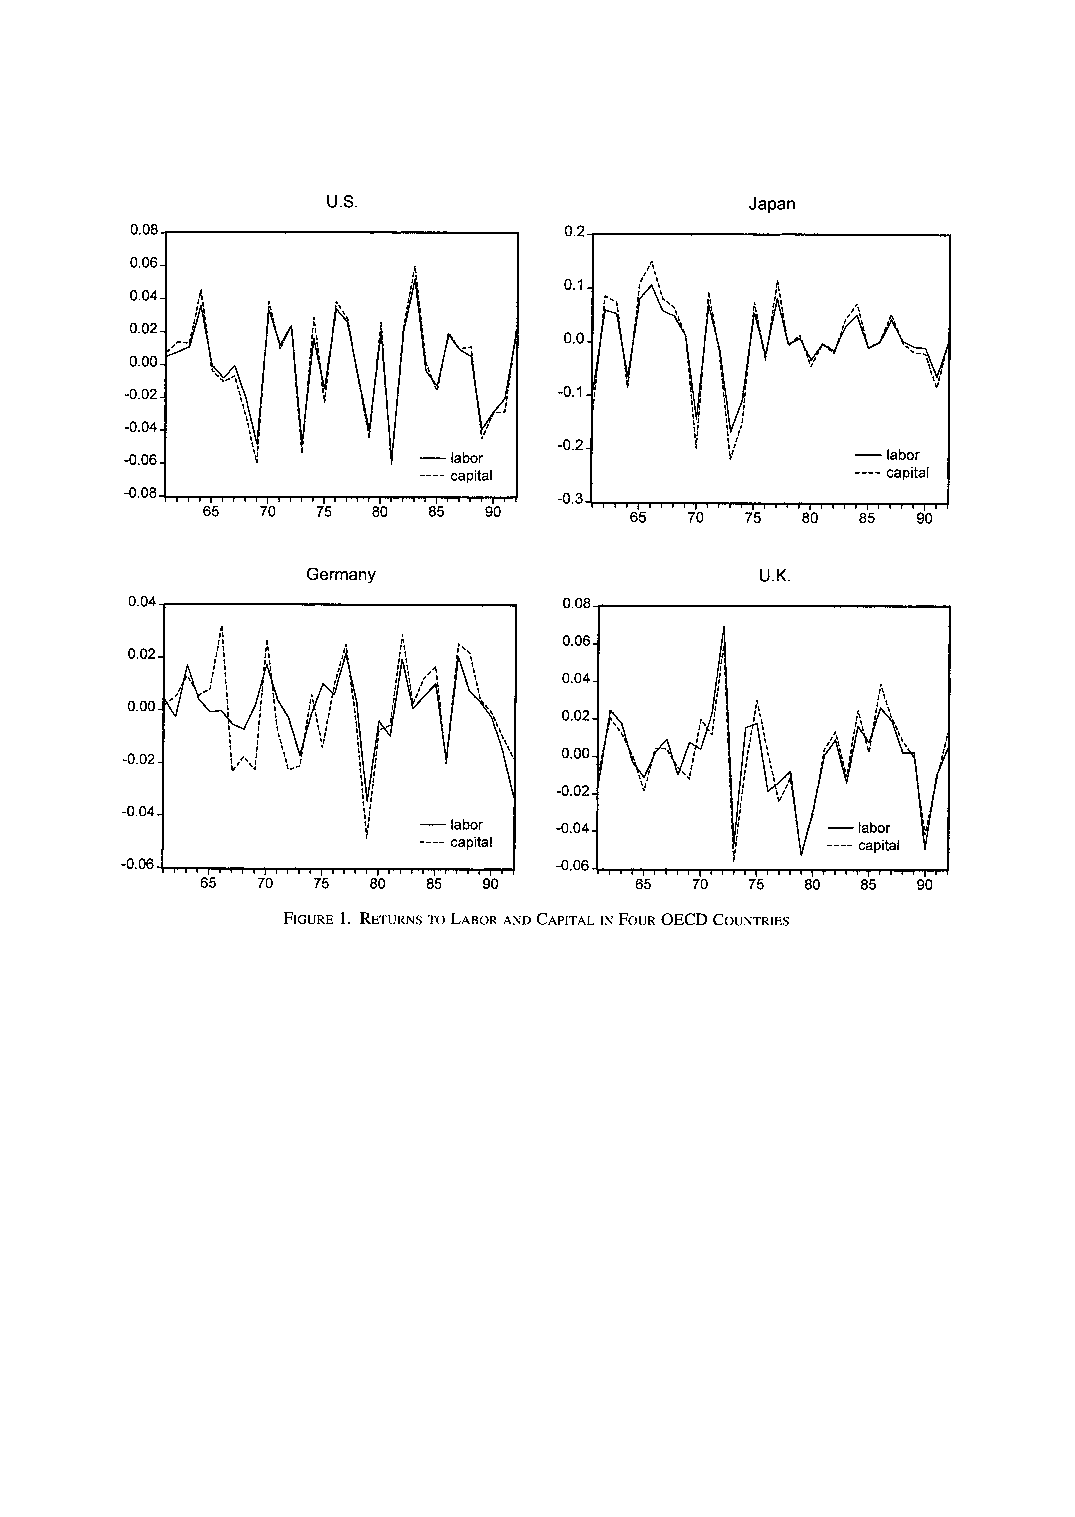
\includegraphics[width=0.8\textwidth]{figure1.pdf}
\end{center}

\end{frame}

\begin{frame}[c]\frametitle{Results II:}

\begin{center}
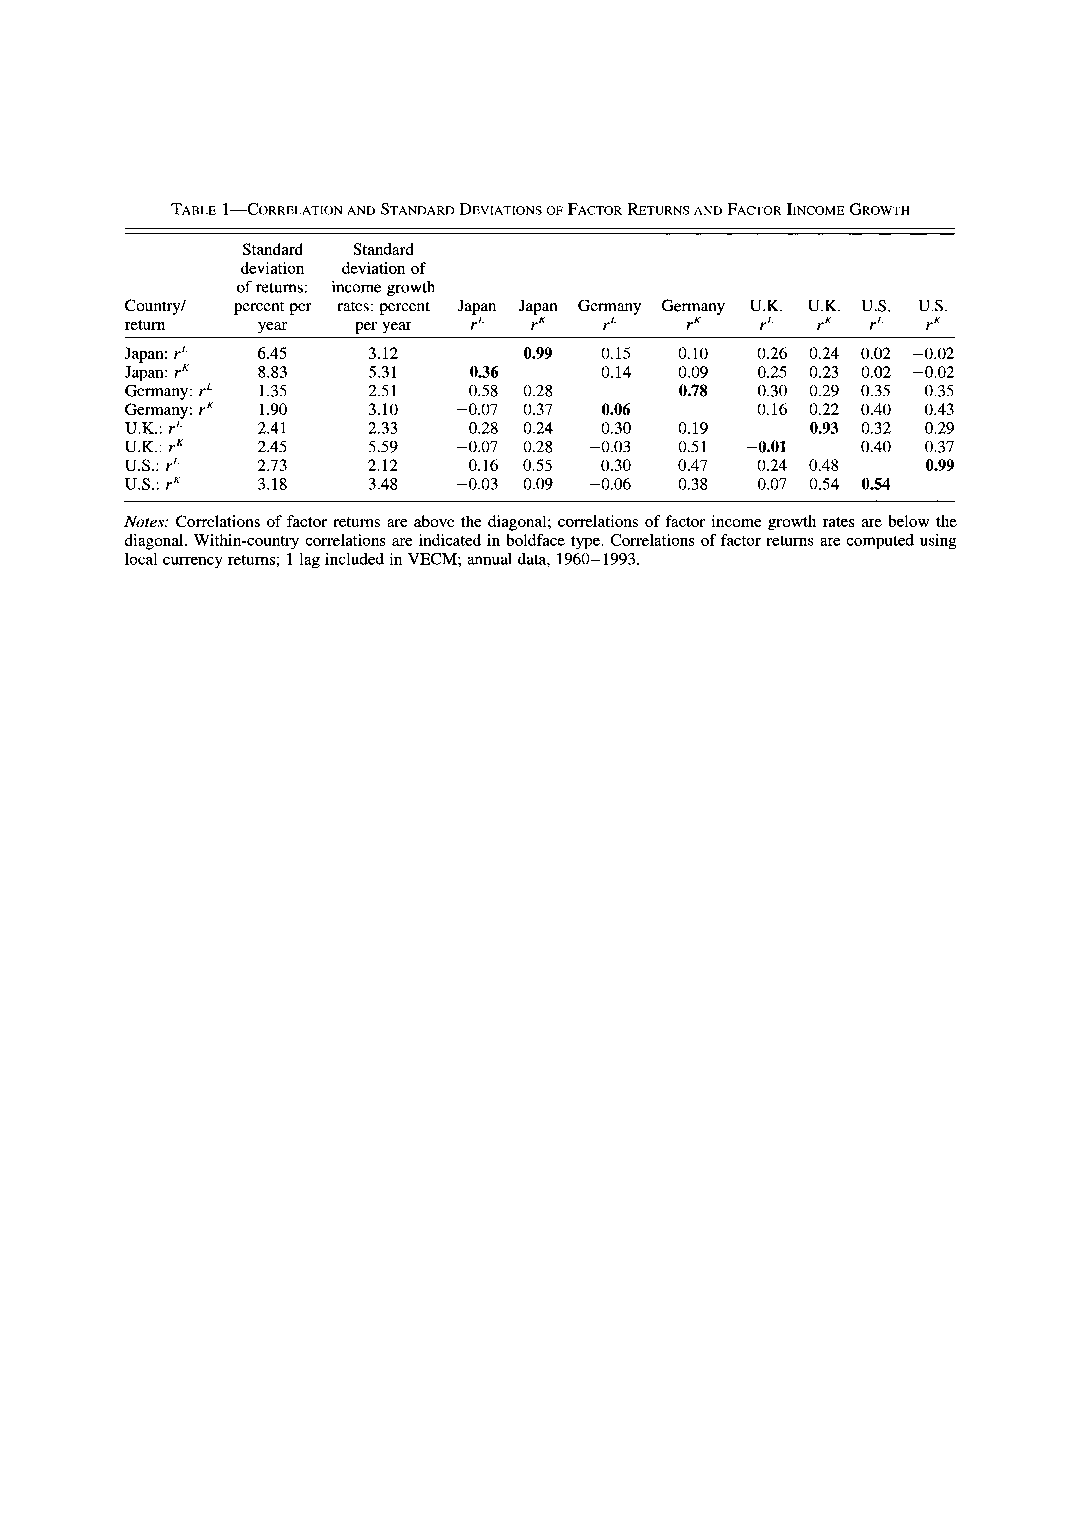
\includegraphics[width=0.95\textwidth]{table1.pdf}
\end{center}
\begin{enumerate}
    \item  labor and capital returns are strongly, positively correlated;
    \item factor returns across countries tend to be not strongly correlated.
    \item the return to labor is less volatile than the return to capital.
\end{enumerate}

\end{frame}

\section[Income V.S. Returns]{Factor Income Growth V.S. Factor Returns}
\begin{frame}[c]\frametitle{Implication}
There is \alert{no necessary relation} btw \alert{growth rates of factor incomes} and \alert{factor returns}.
\begin{itemize}
    \item factor returns can be highly correlated within a country;
    \item growth rates of labor and capital income are much less highly correlated.
\end{itemize}
This is a reflection of the fact that,
\begin{itemize}
    \item In the short term, labor income growth may be largely unrelated to capital income growth.
    \item over the longer term, labor and capital income \alert{share a common stochastic trend}, and it is the trend behavior of factor income growth that dominates factor returns.
\end{itemize}


\end{frame}


\begin{frame}[c]\frametitle{Remarks of Fama and Schwert's argument}
\begin{itemize}
    \item Fama and Schwert (1977) argued that \alert{human capital considerations} were likely to be \textbf{unimportant} for \alert{asset pricing}.
    \item This view is incorrect, the return to human capital is important for asset pricing so long as individuals choose consumption over time in response to market incentives.
   \item Example: wage rate $\Rightarrow$ consumption or not working $\Rightarrow$ productivity of capital $\Rightarrow$ investment decisions.
\end{itemize}
\centerline{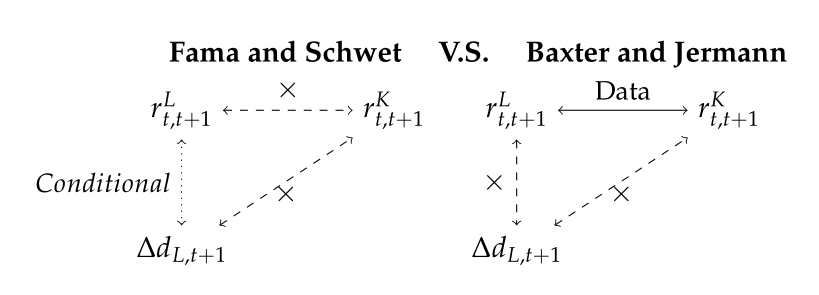
\includegraphics[width=0.8\textwidth]{argu.png}}

\end{frame}

\begin{frame}[c]\frametitle{Special Case:}

Fama and Schwert note that there is one special case in which the growth rate of labor income is the correct measure of the return to human capital.
\begin{enumerate}
    \item $d_{L}$ must follow a random-walk process:
    \begin{equation}
        d_{L,t+1} =  \log(\gamma) + d_{Lt} + \varepsilon_{t+1}
    \end{equation}
    where $\gamma$ is the average growth rate of labor income and $\varepsilon_{t}$ is i.i.d.
    \item the discount factor $\theta$ used to discount future labor income must be constant over time.
\end{enumerate}
The return to human capital is just the growth rate of labor income, up to a constant:
\begin{equation}
    r_{t,t+1}^{L} = \Delta d_{Lt} -\log(\theta \gamma)
\end{equation}


\end{frame}

\begin{frame}[c]\frametitle{Fama-Schwert Regression Again}
Suppose we did run the Fama-Schwert regression in the context of the empirical model of Section II,
\begin{equation}
    \Delta d_{L,t+1} = k_{0} + k_{1} r_{t,t+1}^{K} + u_{t+1}
\end{equation}
\begin{itemize}
    \item $\Delta d_{L,t+1}$ is labor income growth and $r_{t,t+1}^{K}$ is the return to capital that we estimated in Section II.
    \item $k_{1} = 0.22$, with a standard error of 0.12, fail to reject the hypothesis that $k_{1}=0$ at the 5\% significance level.
    \item $\tilde{R}^{2} = 0.07$; the return to capital explains little of the growth rate of labor income.
\end{itemize}


\alert{Explanation}: Labor income growth is not highly correlated with the returns to capital (the correlation is 0.32), even though the  returns to labor are very highly correlated with the returns to capital.
\end{frame}
\section[Implications]{Implications for Hedging Human Capital Risk}
\begin{frame}[c]\frametitle{Hedging Human Capital}

\begin{center}
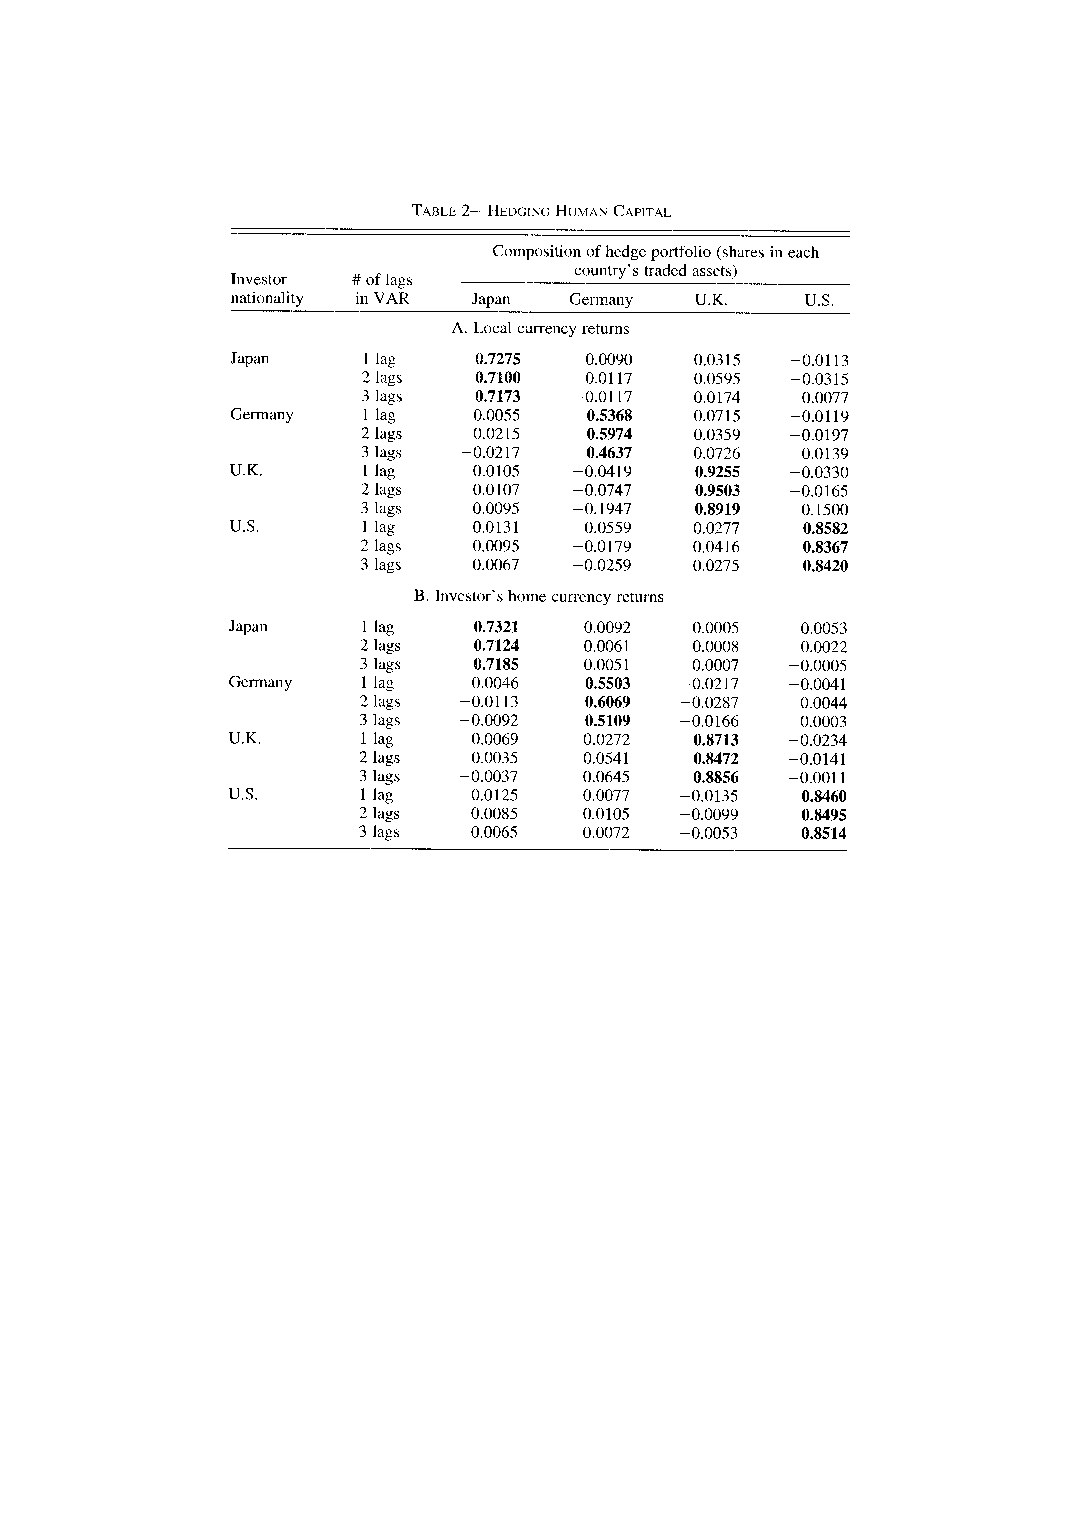
\includegraphics[height=0.85\textheight]{table2.pdf}
\end{center}

\end{frame}

\section[Diversified Portfolio]{Forming a Diversified Portfolio}
\begin{frame}[plain]



\end{frame}
\section{Conclusion}
\begin{frame}[plain]



\end{frame}
\end{document}
